\chapter{Vortex analysis of chaotic, two-dimensional superfluid simulations for few-vortex systems}
\label{ch:2d}

In this chapter, I will describe an application of the GPUE codebase by simulating a two-dimensional system with few vortices that displays chaotic dynamics.
In addition, this chapter intends to highlight the dependence of post-processing metrics such as vortex tracking and the Lyapunov exponent to dynamical studies of superfluid systems.

Chaotic evolution is typically identified by a significant divergence in trajectory based on a small change in the initial conditions~\cite{strogatz2018}, and there have recently been studies into controlling the degree of chaos in quantum systems~\cite{eastman2017, eastman2019}.
For fluid systems, it is possible to induce chaotic behavior in turbulent flow~\cite{spiegel1987, biferale2005}.
For classically turbulent flow, the degree of chaos depends on the Reynolds number~\cite{berera2018}; however, the nature of quantum chaos for superfluid flow is still an active area of research~\cite{white2014}.
Because superfluid vortices have well-defined strength and quantized winding numbers, they can be considered less complex when compared to classical vortices where circulation is continuous; therefore, there has also been significant interest in the differences between classical and quantum turbulence~\cite{nemirovskii1995,kyriakopoulos2014,koukouloyannis2014,navarro2013}.
In spite of the differences between the fluid models, vortex dynamics in superfluid systems are remarkably similar to classical point-vortex models and key features of classical turbulence, such as the Kolmogorov spectrum have been shown to exist for large, turbulent, quantum systems~\cite{nore1997,stalp1999,araki2002,salort2010}.

It is known that it is not possible to easily excite chaotic behavior in large vortex lattices, as these systems have been proven to be stable to many external perturbations~\cite{o2017}.
For this reason, it is interesting to attempt to probe classical chaos in systems with a small number of vortices.
Chaotic, few-vortex systems have been studied previously by Aref and Pomphrey~\cite{aref1982, aref1980, aref1983}, who showed that chaos can be excited in systems with as few as four vortices in an infinite plane~\cite{aref1982}.
Unlike chaos in classical fluids, the onset of chaos in quantum systems seems to appear with fewer vortices present, and few-vortex systems have been explored experimentally for two, three, and four vortices in harmonically trapped BECs~\cite{navarro2013}.
When analyzed with a reduced Hamiltonian approach, harmonically trapped BECs seem to exhibit chaotic effects with as few as three vortices, two co-rotating vortices and an anti-vortex rotating in the other direction~\cite{kyriakopoulos2014,koukouloyannis2014}.
In this approach, the system can be seen as having three degrees of freedom with two integrals of motion, the energy and angular momentum.
This can be further reduced to two degrees of freedom with appropriate canonical transformations and using the angular momentum as a parameter~\cite{koukouloyannis2014}.
For this reason, it seems that three point-vortices is the minimum number necessary for chaotic dynamics.

Experimentally, it is now possible to detect vortex circulation~\cite{seo2017} and image vortices in-situ~\cite{wilson2015}.
It is also possible to probe vortex dynamics at different times within a single experiment~\cite{freilich2010, serafini2017}.
Because quantum vortices are simple and BECs are highly controllable experimental systems that can be restricted to two dimensions, there has been significant interest in two-dimensional quantum turbulent systems as well~\cite{neely2013,shin2004}.
Additional effects, such as the K\'arm\'an vortex street~\cite{kwon2014} and Onsager vortex clusters~\cite{gauthier2018,johnstone2018} have already been shown to exist experimentally.

Because chaotic events require very small changes in the initial conditions of the system, it is important to create a system with well-controlled initial conditions.
For this, I will start with a small vortex lattice of four vortices, and then create a defect in this lattice using phase imprinting, as described in Chapter~\ref{ch:splitop}.
This process will controllably induce chaotic vortex dynamics in an experimentally feasible way.
We also show that the chaotic dynamics are enhanced by the close approach of vortices.

The content of this chapter has been published in \textit{Phys. Rev. Fluids} (\textbf{4}(5):054701, 2019), and for this work, I oversaw the simulations performed by Tiantian Zhang and developed the GPUE codebase to allow for the phase imprinting methods necessary to generate the chaotic vortex behavior described in this study.
This work had two separate advisors, Thomas Busch and Angela White, who both directed the physics and helped interpret the results.

\section{Model}

The physics simulated in this Chapter is purely two-dimensional, so it is appropriate to begin this section with a disclaimer about the dimensionality of the system I will be simulating.
In principle, all real-world physics is three-dimensional, but just as a one-dimensional cigar-shaped BEC can be created, a pancake-like geometry can also be constructed by increasing the trapping frequency in the $\hat z$ (perpendicular) direction with respect to the $\hat x$ and $\hat y$ (transverse) directions.
With this geometry, one can assume that the condensate is in the ground state along the $\hat z$ dimension so long as any excitations in the $\hat z$ direction requires an energy larger than the chemical potential.
One can then factorize the wavefunction as $\Psi(\mathbf{r},t) = \Psi(x, y, t)\phi(z)$, where $\Psi(x, y, t)$ is the wavefunction in the transverse plane and $\phi(z) = (m \omega_z/(\pi\hbar))\text{exp}(z^2 m\omega_z/(2\hbar))$ is the ground state along the $\hat z$ dimension.
By integrating over $\hat z$, the interaction strength is modified for a two-dimensional condensate to be
\begin{equation}
g_{2D} = g \sqrt{\frac{m\omega_z}{2\pi\hbar}}.
\end{equation}
\noindent With these changes, one can simulate two-dimensional settings with the GPUE codebase~\cite{zhang2019, o2017, o2016topo, o2016}.
This chapter will apply several of the techniques mentioned in Chapters~\ref{ch:splitop} and \ref{ch:gpu} to a rotating two-dimensional BEC system for a small number of vortices.

\begin{figure}
\center 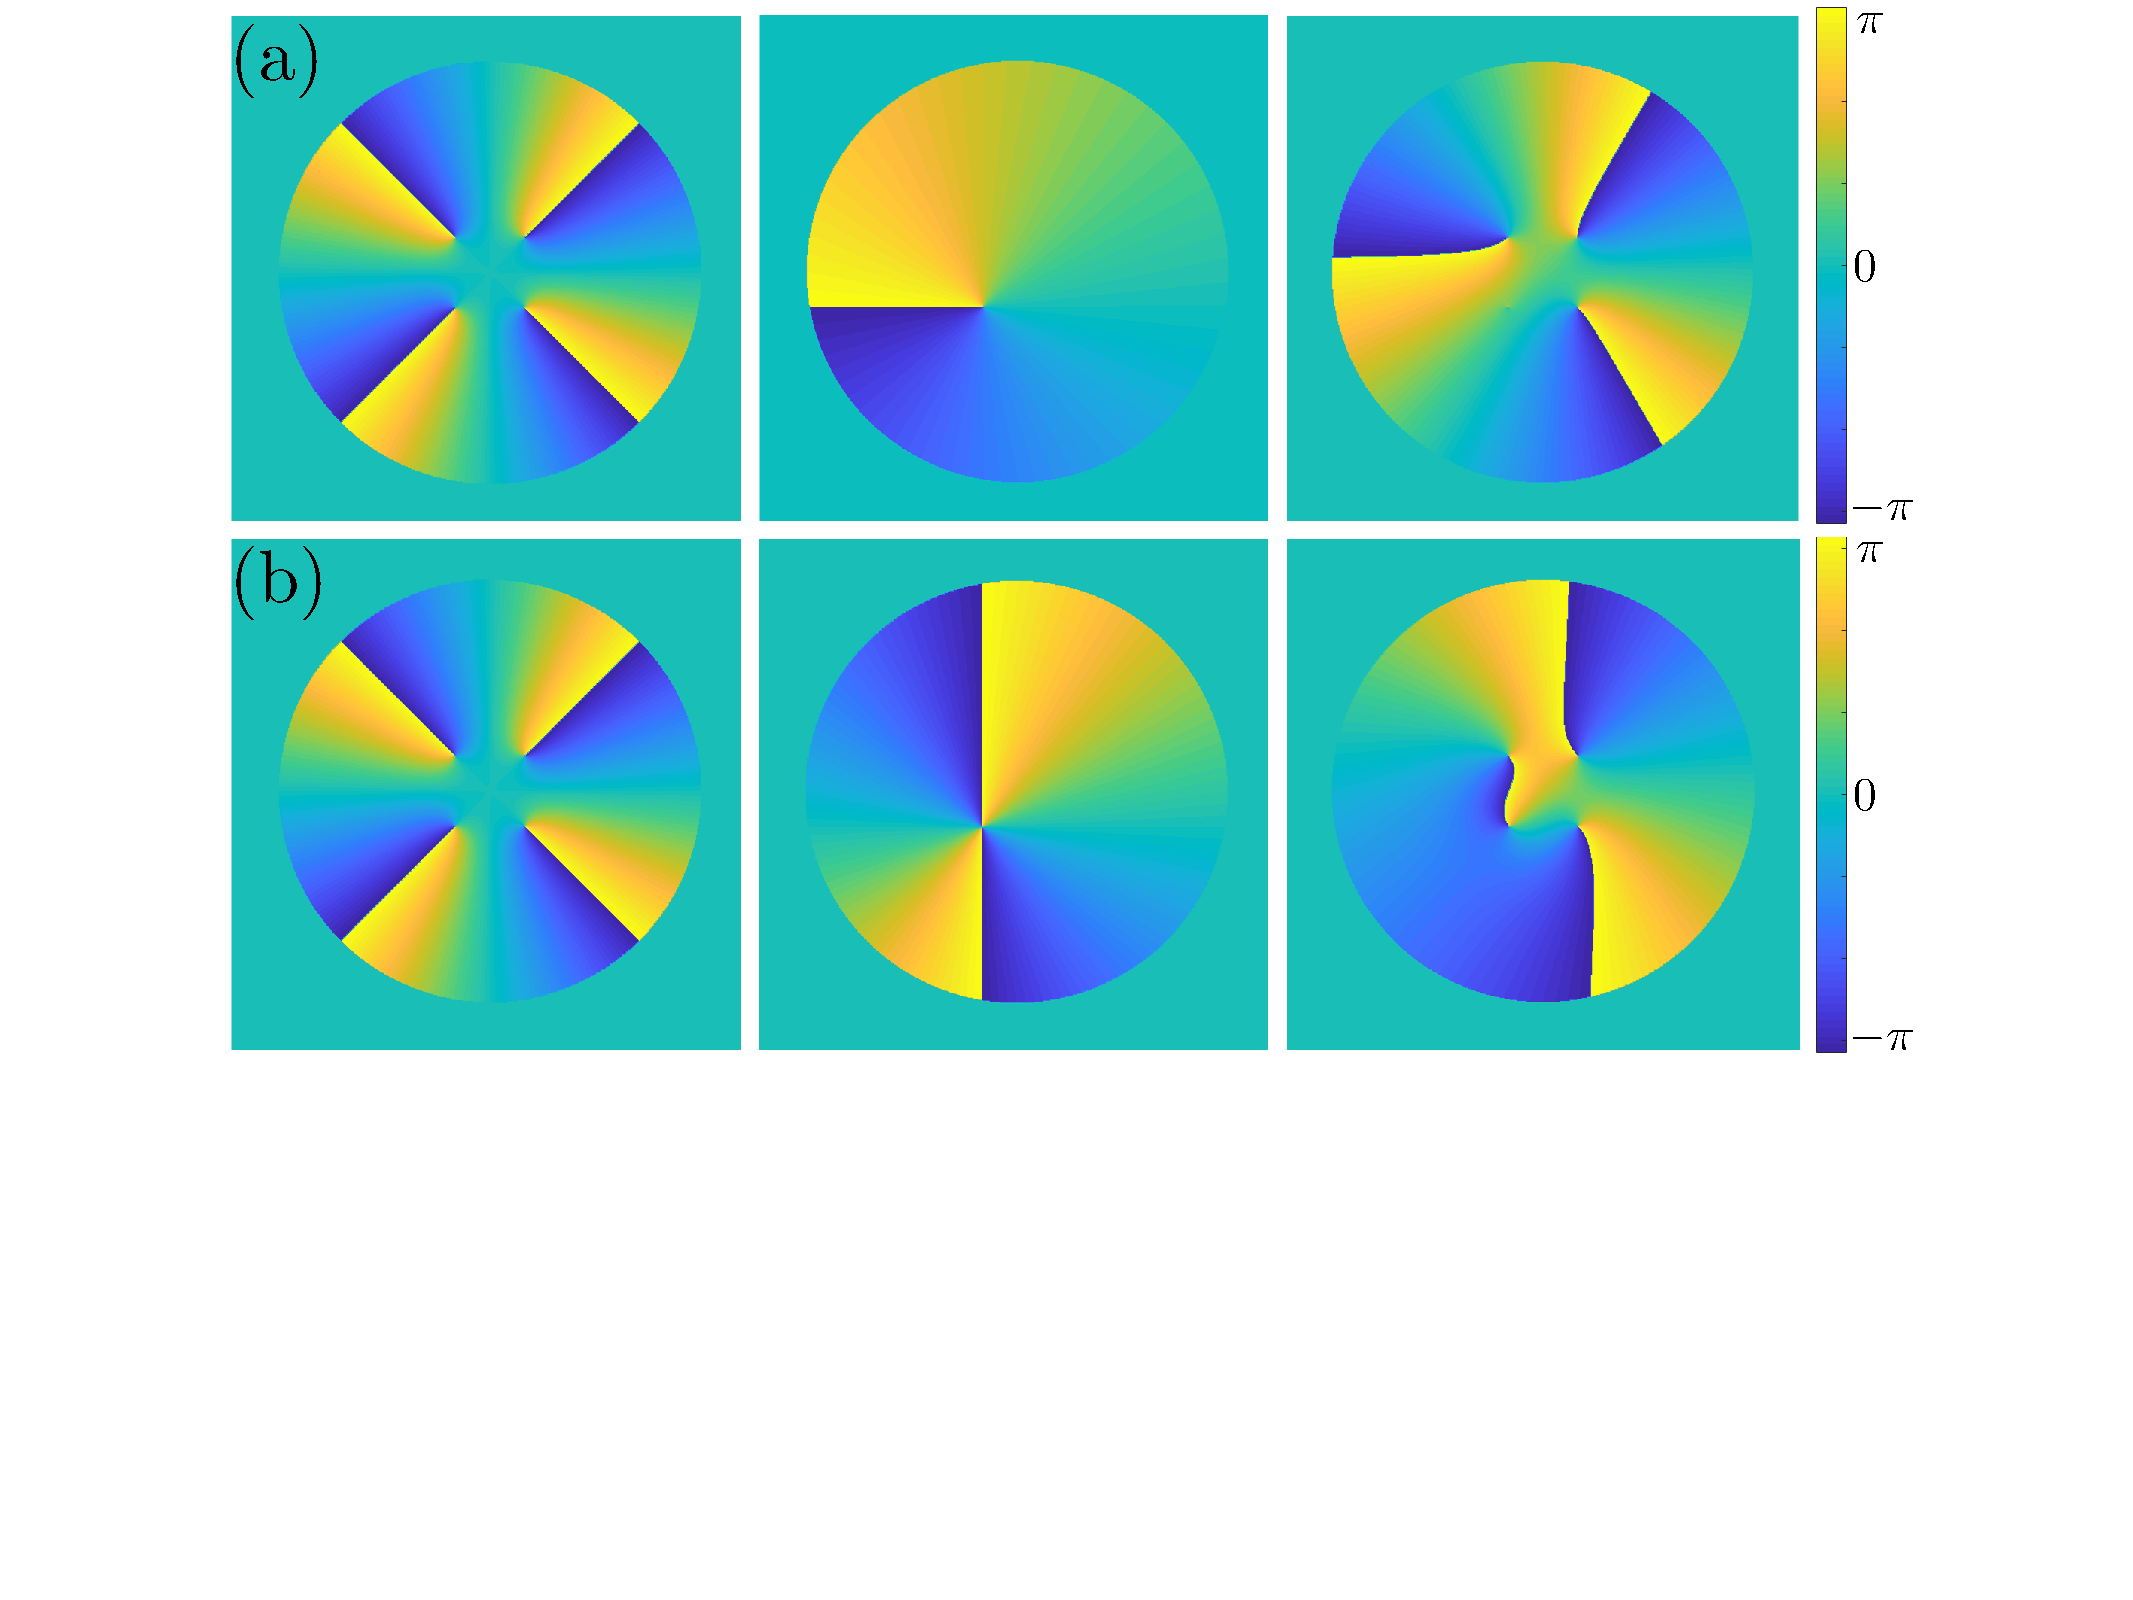
\includegraphics[width=0.75\textwidth]{data/2d/phase/phase}

\caption{
Phase distribution of the initial four co-rotating vortex system is shown at the left.
In the center is the applied phase mask of $-2\pi$ for (a) and $-4\pi$ for (b), and the resulting phase distribution is shown on the right.
By applying a $-2\pi$ phase winding, a vortex is erased from the system, and by applying a $-4\pi$ phase winding, the vortex is flipped, creating an anti-vortex.
}
\label{fig:phase}
\end{figure}

For this study, a condensate with $N = 10^6$ $^{87}$Rb atoms in the co-rotating frame with an s-wave scattering length of $a_s=4.76\times 10^{-9}$m in a pancake geometry with typical trapping frequencies of $(\omega_\perp, \omega_z) = (2\pi, 32\pi)$ Hz will be considered.
Here, the effective two-dimensional interaction strength is $g = 6.8\times 10^{-40}$ m$^4$kg/s$^2$.
These simulations were performed on a grid of $2^{10} \times 2^{10}$ points and covering an extent of $700\mu \text{m} \times 700 \mu \text{m}$

Although large rotational frequencies will create a triangular lattice, for smaller frequencies, other configurations are known~\cite{aftalion2001}, and I will focus on the regime where the ground state is composed of four vortices in a square configuration~\cite{zampetaki2013}.
Once this configuration is achieved, one vortex is manipulated via phase imprinting, such that three co-rotating vortices and one anti-vortex exist in the system.
Examples of phase imprinting on this system can be seen in Figure~\ref{fig:phase}, where the top row shows a simple vortex annihilation and the bottom row shows a vortex flip.

\section{Regular and irregular vortex dynamics}

\begin{figure}
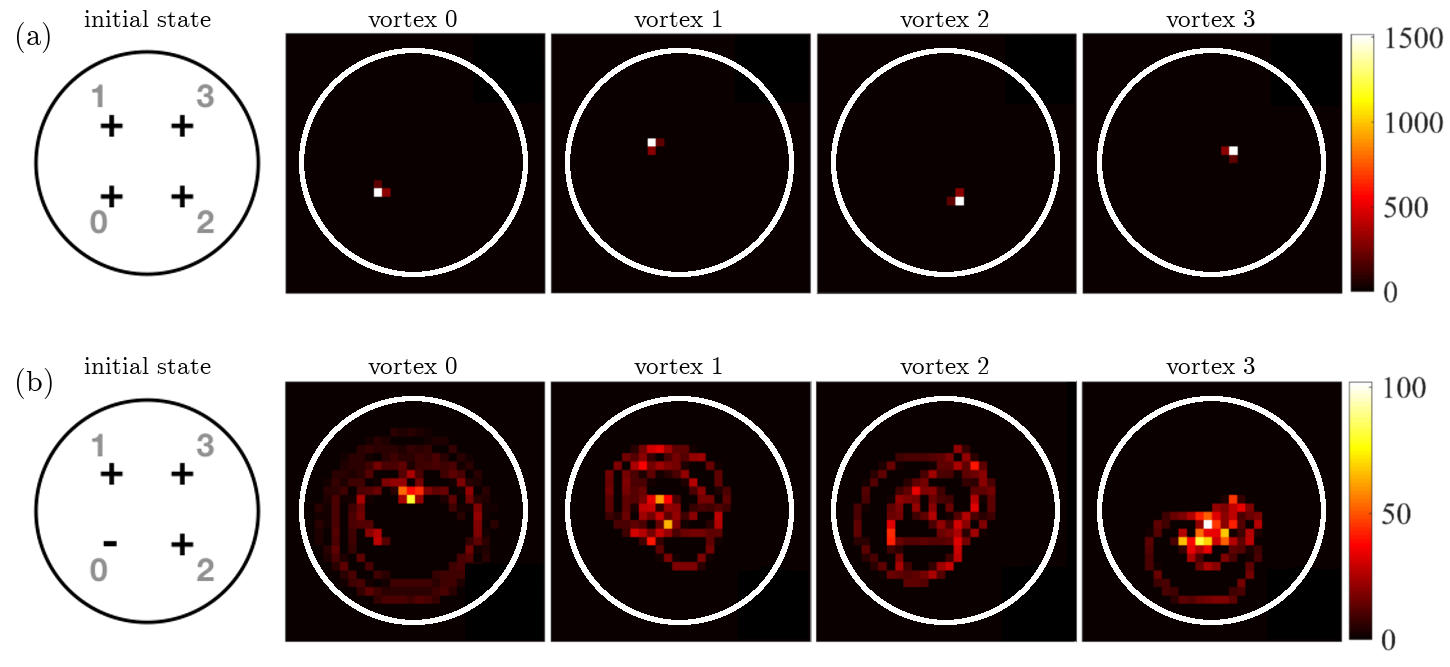
\includegraphics[width=\textwidth]{data/2d/histogram/histogram}

\caption{
Histograms of the positions of each vortex in the transversal plane for 20 seconds in the co-rotating frame.
The lower left vortex has been annihilated and re-imprinted with (a) the same and (b) the opposite direction of rotation, exactly on the location of the previous vortex.
The area of each plot is $400\mu \text(m) \times 400 \mu \text{m}$, and the white circles correspond to iso-lines at 40\% of the maximum density to highlight the extent of the vortex motion.
In (a), if all four vortices are co-rotating, regular trajectories appear, but in (b), flipping the rotation direction of a single vortex creates disordered trajectories.
}
\label{fig:histogram}
\end{figure}

It is known that a lattice of vortices with the same direction of rotation will exhibit regular dynamics~\cite{abo2001}, and this is confirmed in Figure~\ref{fig:histogram}(a).
In this figure, I show a histogram of the vortex trajectories over 20 seconds of evolution when removing and then re-imprinting a vortex of the same rotational direction at the same location.
Even though a small residual movement appears, potentially due to phonon excitations that were not fully removed from the imaginary time evolution, the vortices remain stationary.
In Figure~\ref{fig:histogram}(b), I also show that if the re-imprinted rotation is of the opposite direction, the vortex dynamics become more disordered, with vortices traversing a larger width of the condensate.
It is worth mentioning that similar histograms can be constructed experimentally with available imaging techniques~\cite{wilson2015,freilich2010}.

\begin{figure}
\center 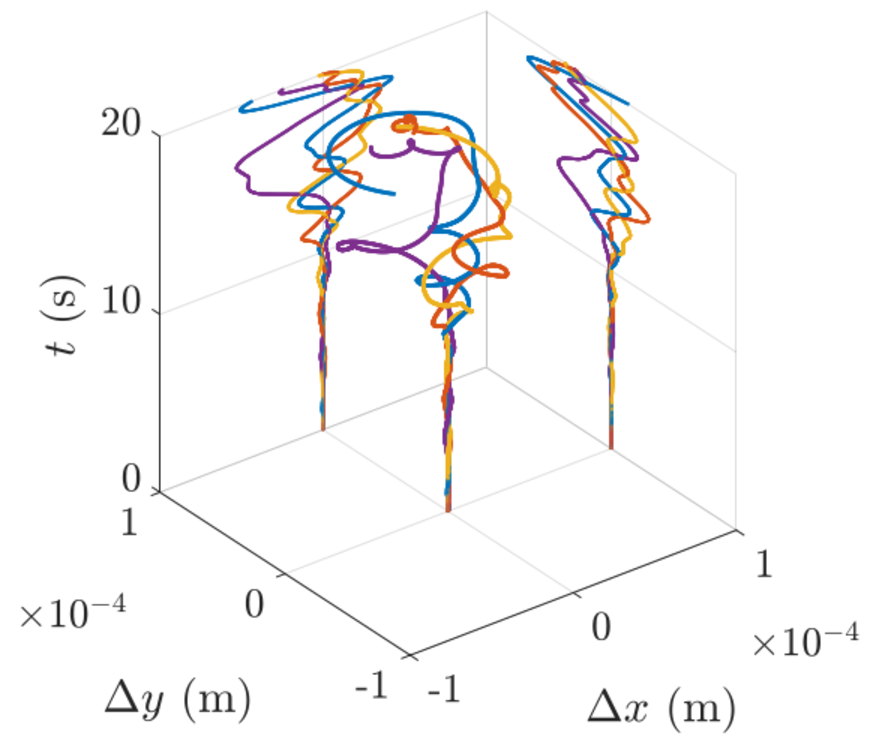
\includegraphics[width=0.5\textwidth]{data/2d/evolution/evolution}

\caption{
Evolution of the difference in trajectories $\triangle \textbf{r}_i = \textbf{r}_{i}-\textbf{r}'_{i}$ with $\textbf{r}$ corresponding to the position of the $i$th vortex from the center of the condensate and $i\in \{0,\ 1,\ 2,\ 3\}$ labelling each individual vortex for the four-vortex system as shown in Fig.~\ref{fig:histogram}.
A small change in the initial position of the anti-vortex arises from a phase-imprint at $(x_{0},y_{0})$ and $(x_{0}-\xi/3,y_{0})$ where $(x_{0},y_{0})$ denotes the pre-existing co-rotating vortex core position.
The curves show that even though the onset of disorder is immediate, a strong divergence of trajectories is observed at about $t\approx 10 \text{s}$ (see projections onto the $x$-$t$ and $y$-$t$ planes).
The difference in trajectory of the anti-vortex, $\Delta \mathbf{r}_0$, is shown in blue, while yellow, orange, and purple lines depict the three co-rotating vortices.
}
\label{fig:evolution}
\end{figure}

Even though the introduction of the anti-vortex creates disordered trajectories, it could be entirely possible that these trajectories are still stable.
To uniquely identify chaotic behavior, one needs to show that any small perturbation in the vortex location will also provide a significantly different trajectory.
To check this, two sets of vortex trajectories are compared with slightly different shifts in the initial position of the anti-vortex, $\mathbf{r}_0$ and $\mathbf{r}'_0$, where $\mathbf{r}_0 - \mathbf{r}'_0 = \xi/3$ and $\xi$ is the healing length.
In Figure~\ref{fig:evolution}, I show the differences in trajectories, defined as $\Delta \mathbf{r}_i(t) = \mathbf{r}_{i}(t)-\mathbf{r}'_{i}(t)$, where $\mathbf{r}_i$ refers to the position of the $i$th vortex from the center of the condensate and $i\in \{1,2,3\}$ corresponds to the vortex number.
The unique index for each vortex is shown in Figure~\ref{fig:histogram}.
Here, one sees that the difference in trajectories is initially small, but diverges significantly at around $t \approx 10$ seconds, which is a strong indication of chaotic behavior.

After closely inspecting the vortex dynamics (shown in the supplementary movie~\cite{movie}), one sees that this strong divergence in vortex trajectories seems to be accelerated when all four vortices come in close proximity.
Because the velocity fields of each vortex decays as $1/\mathbf{r}$, where $\mathbf{r}$ is the distance from the vortex's core, the vortices experience stronger velocity fields when they are closer; therefore, the point of minimal separation can be seen as a highly nonlinear multi-vortex scattering event that accelerates the divergence shown in Figure~\ref{fig:evolution}.
In Figure~\ref{fig:snapshots} this is studied further by showing snapshots of the condensate density before ($t = 6$s), at ($t = 10$s), and after ($t = 15$s) the scattering event in (a) and (b) for the non-shifted and shifted initial anti-vortex locations.
The differences between position of each vortex and the anti-vortex is also shown (c) for the case where the anti-vortex is shifted by $\xi/3$.
Here, there is a clear minimum at $t \approx 10$ seconds, which is the same time at which the  trajectories begin to diverge in Figure~\ref{fig:evolution}.
In order to characterize this divergence in trajectory, one must analyze the vortex dynamics in more detail by calculating (for example) the Lyapunov exponent.

\begin{figure}
\center 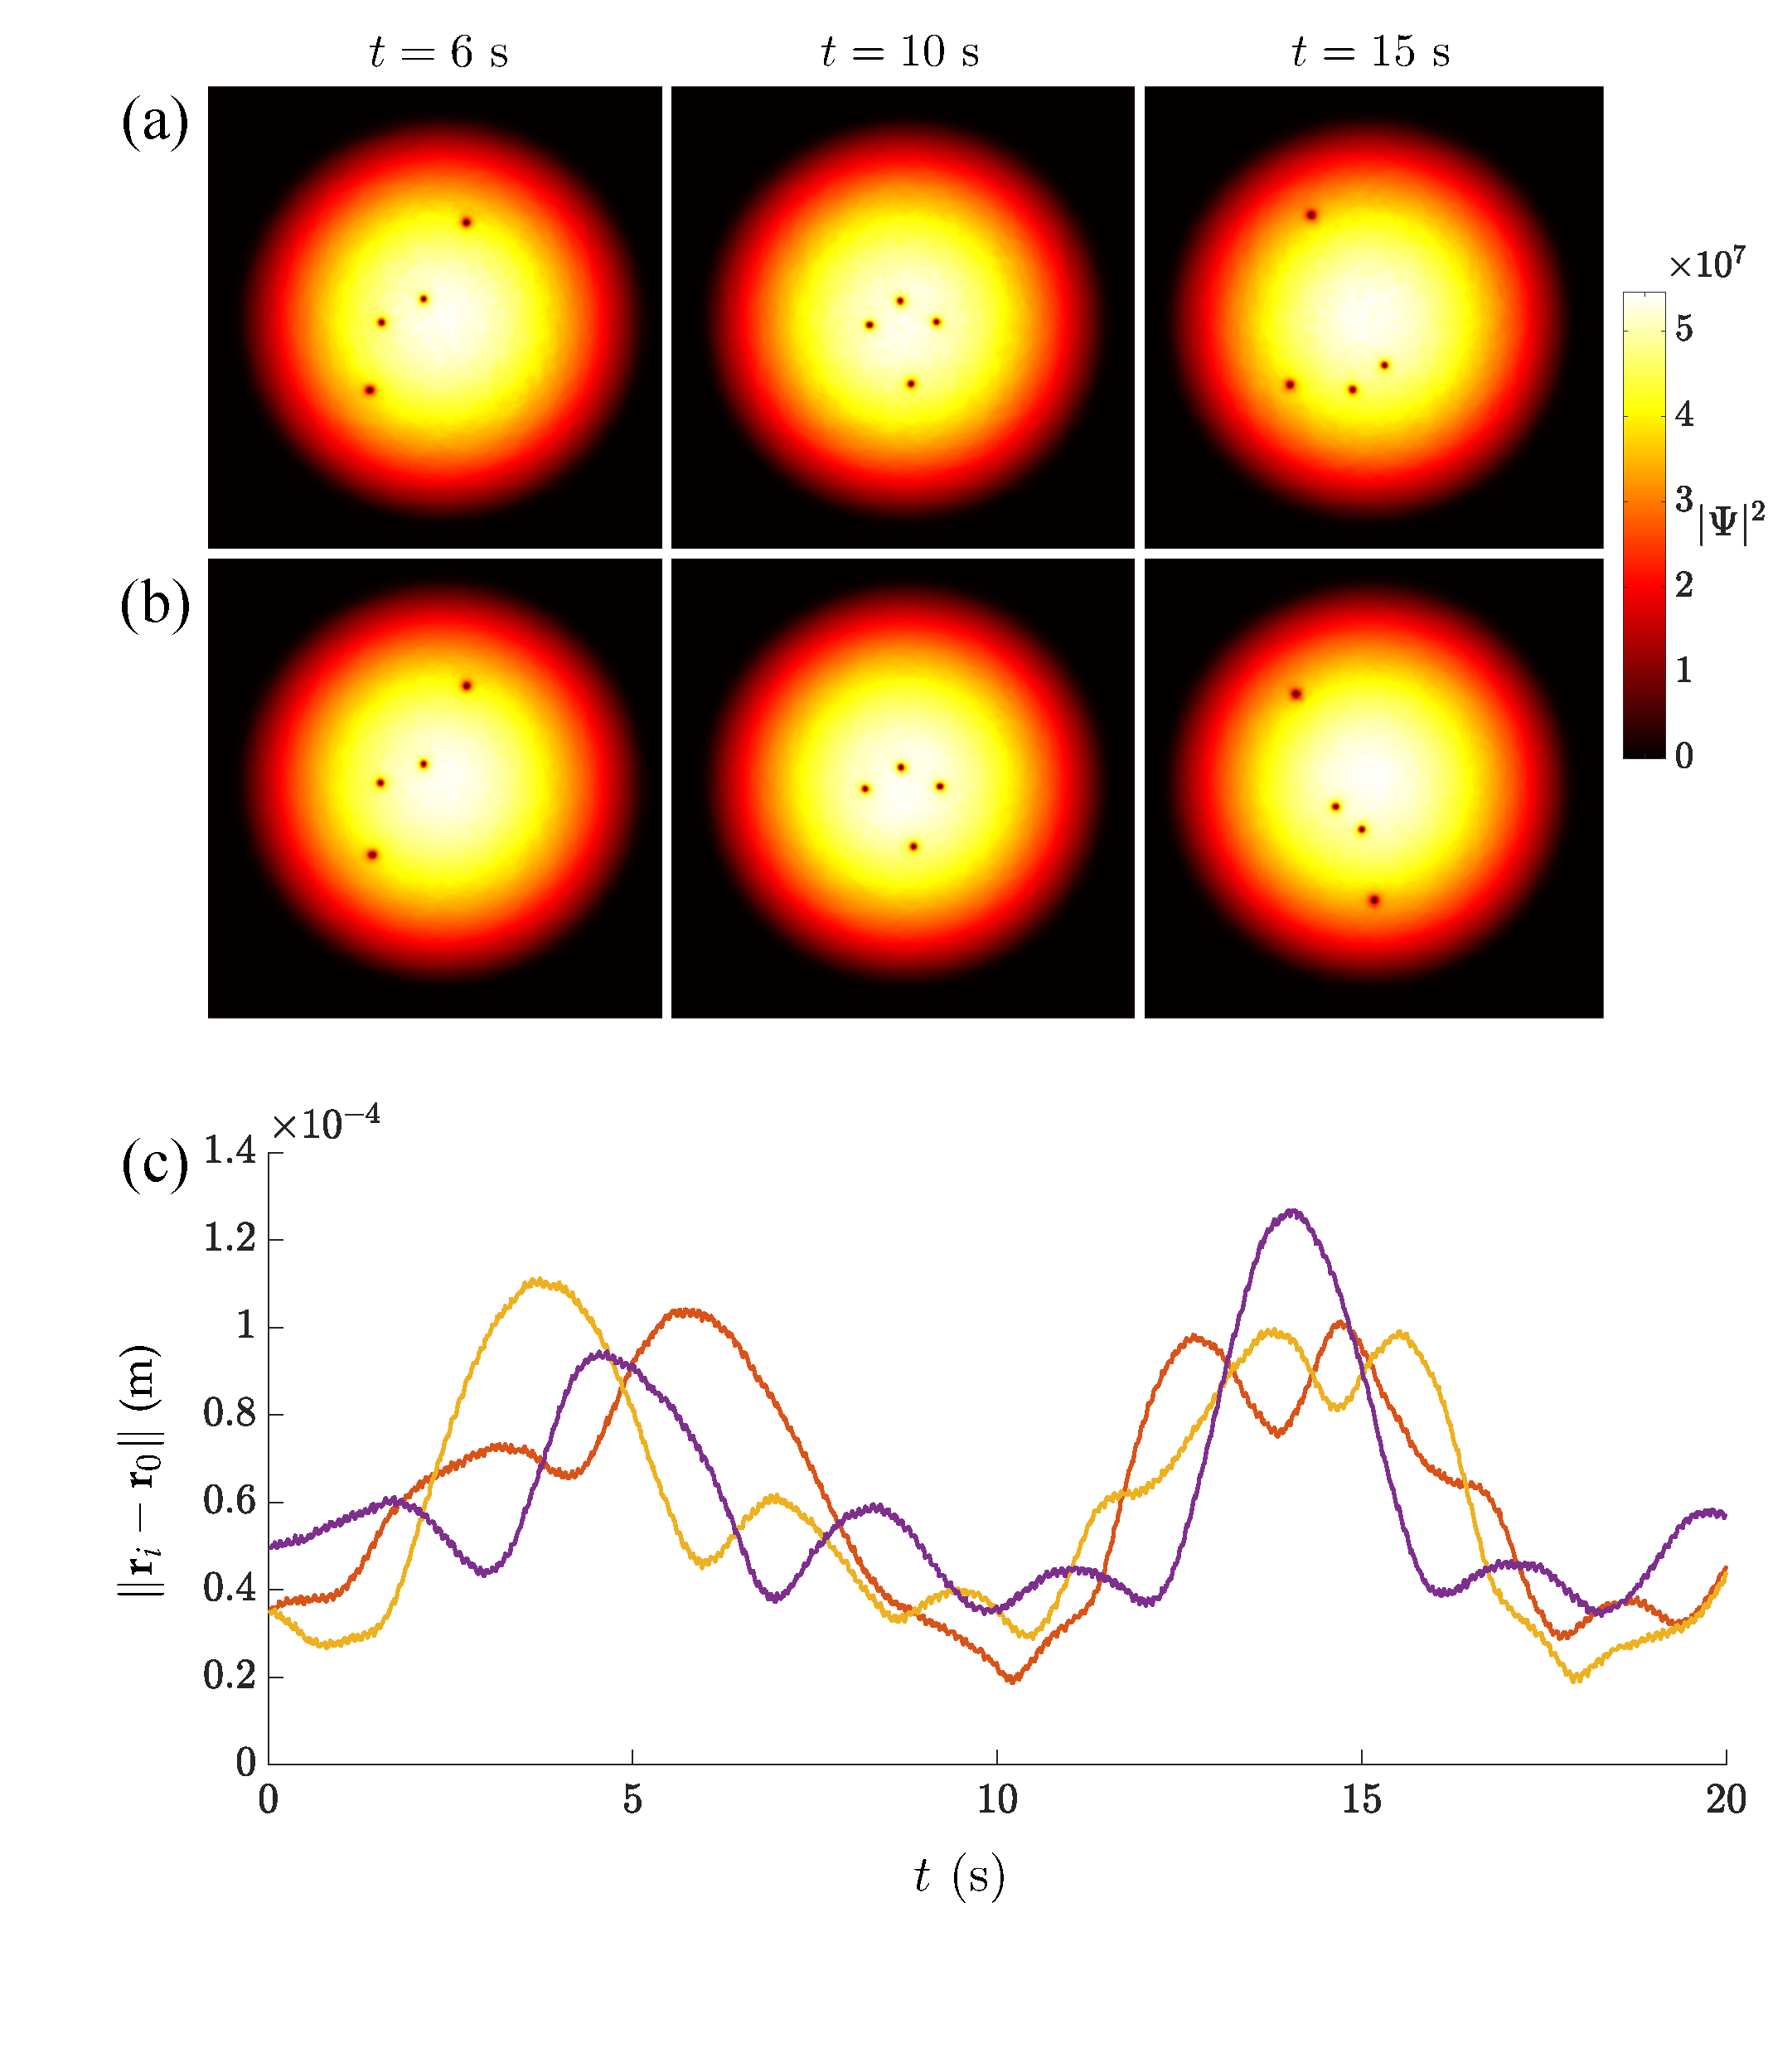
\includegraphics[width=0.75\textwidth]{data/2d/snapshots/snapshots}

\caption{
Density plots of condensate for (a) $\Delta x = 0$ and (b)$\Delta x=\xi/3$ at times $t=\{6,10,15\}$ s. The densities before the scattering event differ only on small scales (see $t=6s$), whereas for times after the event, large deviations are visible (see $t=15s$).
At $t=10$ seconds the vortices make their closest approach. The area plotted is $500 \mu m\times 500 \mu m$.
(c) Distances between the vortices at positions $\mathbf{r}_i$ with $\mathbf{r}$ corresponding to the position of the $i$th vortex from the center of the condensate and $i\in \{1,2,3\}$ corresponding to the vortex number as shown in Fig.~\ref{fig:histogram} and anti-vortex at $\mathbf{r}_0$ for $\Delta x = 0$.
A minimum around $t=10$ seconds is clearly visible.
}
\label{fig:snapshots}
\end{figure}

\section{Characterizing chaotic vortex dynamics}

\begin{figure}
\center 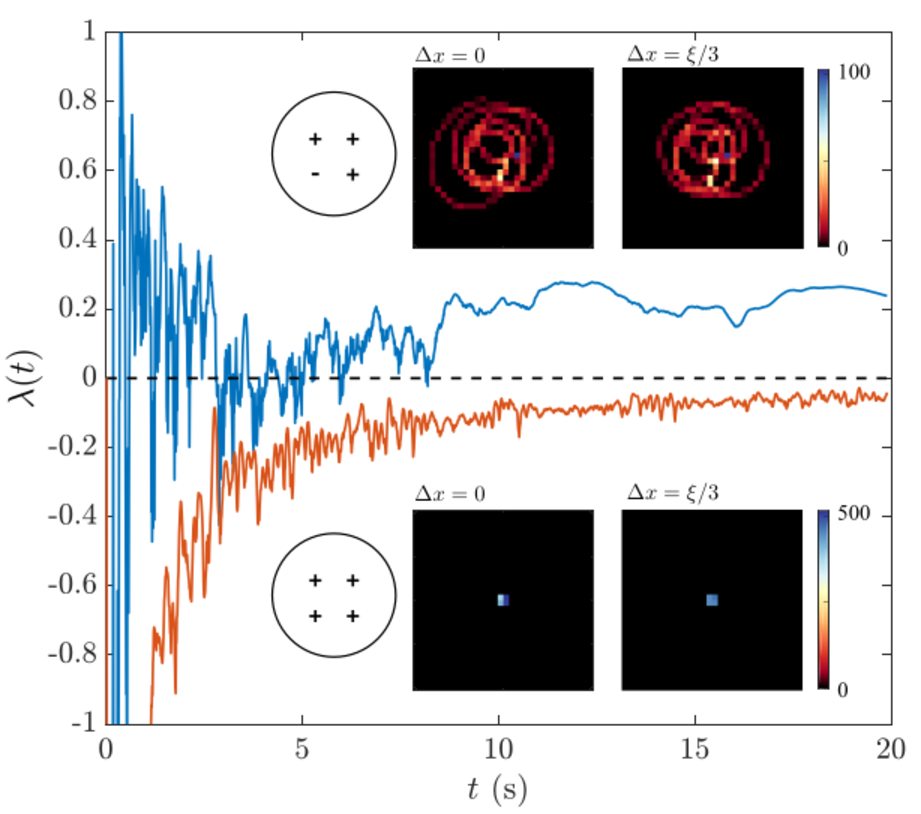
\includegraphics[width=0.75\textwidth]{data/2d/lyap/lyap}

\caption{
The insets show the histograms of the COM trajectories calculated over 20 seconds of evolution for the system of four vortices when the position of a single vortex has been shifted by $\Delta x=0\xi$ and $\Delta x=\xi/3$.
The upper two panels depict the corresponding trajectories after the direction of rotation of a single vortex has been reversed, whereas the lower row displays the trajectories for the case where all vortices co-rotate.
The main curve plots the corresponding time-dependent Lyapunov exponents,  calculated from the shown COM trajectories. 
The negative time-dependent Lyapunov exponents (orange) indicate that shifting the vortex about the initial position still ensures the stability of vortex trajectories. Reversing the direction of circulation of a single vortex (blue) however leads to fluctuations about zero, eventually leading to a fully positive exponent. 
}
\label{fig:lyap}
\end{figure}


To characterize the degree of chaos for the shown vortex dynamics, a variation on Lyapunov exponents will be used.
These exponents give the rates of divergence for nearby orbits in phase space~\cite{wolf1985},
and with this measure, one can track two trajectories in phase space to see if the divergence between the two trajectories will either exponentially converge or diverge, which can be modeled with

\begin{equation}
|\delta\mathbf{Z}(t)| \approx e^{\Lambda t} |\delta \mathbf{Z}_0|.
\end{equation}

\noindent Here, $\delta\mathbf{Z}_0$ is the initial separation between the trajectories and $\Lambda$ is a quantity known as the Lyapunov exponent.
If the exponent is negative, this means that the trajectories tend to converge, but if it is positive, the trajectories will diverge, thus indicating chaotic motion.
The rate of divergence is determined by the value of the exponent.

For this simulation, trajectories are modeled in four-dimensional phase-space with $\mathbf{P(t)} = (x(t), y(t), v_x(t), v_y(t))$ and $\mathbf{P}'(t) = (x'(t), y'(t), v'_x(t), v'_y(t))$.
The separation is then defined to be $\delta \mathbf{P(t)} = (\delta x(t), \delta y(t), \delta v_x(t), \delta v_y(t))$ where $\delta x(t) = x(t) - x'(t)$, etc.
The exponent can then be calculated as

\begin{equation}
\Lambda = \lim_{t\to\infty}\frac{1}{t}\text{ln}\frac{||\delta\textbf{P}(t)||}{||\delta\textbf{P}(0)||}
\label{eqn:lyap_full}
\end{equation}

\noindent where $||\cdot||$ denotes the Euclidean norm.

Because this system is finite, the value of the Lyapunov exponent from Equation~\eqref{eqn:lyap_full} will tend to 0.
For this reason, rather than performing the full calculation of the Lyapunov exponent, $\Lambda$, I will instead show the exponent as a function of time, here notated as

\begin{equation}
\lambda(t) = \frac{1}{t}\text{ln}\frac{||\delta\textbf{P}(t)||}{||\delta\textbf{P}(0)||}.
\label{eqn:lyap}
\end{equation}

\noindent This value can characterize chaotic dynamics in finite-sized systems, and
will be referred to as the time-dependent Lyapunov exponent for the remainder of this work.

In this case, each vortex is tracked with the methods outlined in Chapter~\ref{ch:gpu}, which use both the position and velocity of the vortex.
To determine whether the total system is chaotic, beyond its constituent vortices, I use a center of mass (COM) variable, defined as $\mathbf{R}_M = \frac{1}{n+1}\sum_{i=0}^nr_i$, where $n+1$ is the number of vortices.
Similarly, the center of velocity is defined as $\mathbf{v}_M = \frac{1}{n+1}\sum_{i=0}^nv_i$.
These values are then used with Equation~\eqref{eqn:lyap}, and the results are shown in Figure~\ref{fig:lyap}.
The insets in Figure~\ref{fig:lyap} show the histograms of the COM trajectories for the case where an anti-vortex is and is not present.

As expected, the exponent spectrum calculated in Figure~\ref{fig:lyap} shows that the regular, co-rotating system always shows a negative (converging) exponential value, but the system with the anti-vortex is largely positive (diverging).
During the scattering event shown in Figures~\ref{fig:snapshots} and \ref{fig:evolution}, the exponent becomes positive for the remaining duration of the simulation.
It is worth noting that other global measurements could be used instead of the COM, such as the center of charge~\cite{kyriakopoulos2014}, but these were found to provide similar qualitative results to those shown here.


\section{Outlook}

With this study, I have shown that it is possible to induce chaotic vortex dynamics in a two-dimensional few-vortex systems by using phase imprinting to flip the rotational direction of a vortex.
I also show that a scattering event seems to be correlated to a positive time-dependent Lyapunov exponent and an acceleration of chaotic behavior.
This behavior is radically different to the behavior of large scale vortex lattices, where similar techniques have been shown to only cause local disturbances~\cite{o2016topo}.
Further exploration of the crossover from regular to turbulent dynamics, and the crossover from chaotic to stable dynamics for large-scale vortex lattices remains an interesting extension for future work.

This study shows that there is strong utility in simulating two-dimensional quantum gases and highlights dynamic measures, such as the Lyapunov exponent.
Here, it is obvious that fast vortex tracking methods are essential to dynamical turbulence and chaos modelling, and a major limitation to performing similar studies in three dimensions is the computational hurdle of vortex tracking in this area.
As such, most three-dimensional studies of quantum chaos rely on other methods, such as vortex filament methods which provide vortex skeletons during the simulation, itself.
As mentioned in Chapter~\ref{ch:splitop}, these methods cannot simulate the underlying dynamics of the condensate, and are thus removed from experimental application.
Further extensions of this work in three dimensions would also allow for studies on the movement of the vortex lines, themselves, which were projected onto two-dimensional point-vortices in this model.

It is important to note the utility of the GPUE codebase in this study.
Throughout the process, highly-resolved (up to $2048 \times 2048$) wavefunction densities were generated in the ground state via imaginary time propagation and dynamics were determined with real-time evolution.
For a typical run of $1024 \times 1024$ with $1\times 10^6$ steps, with a time resolution of $1\times 10^{-5}$ and outputting every 1000 steps, the simulation can be completed within an hour.
This metric includes vortex tracking on every output step, which is a computational intensive task, as discussed in Chapter~\ref{ch:gpu}.
Because of the computational speed of GPUE, this study performed hundreds of individual runs with slightly varying initial conditions to provide a strong indication of chaotic behavior.
Because this study very heavily relied on post-processing metrics, such as vortex tracking and the calculation of the Lyapunov exponent, it is apparent that it is ideal to provide an interface to the GPUE codebase in a language that more easily provides the functionality expected by researchers for data manipulation.
Such an interface is possible with GPUE.jl and further motivates this development.

For the next study, I will transition into a discussion of three-dimensional vortex dynamics and show an experimentally realistic system to allow for the generation, control, and detection of vortex ring-like systems with artificial magnetic fields.


